% Chapter 8 --- Results and Expert Validation

\chapter{Results and Expert Validation}\doublespacing
\label{Chapter8}
\lhead{Chapter VII. \emph{Results and Expert Validation}}

%----------------------------------------------------------------------------------------
\section{Introduction}
%----------------------------------------------------------------------------------------

% Note to author: This chapter should be completed following the conclusion of the
% June field trials at the five factory locations. The sections below provide the
% structural framework and describe the validation methodology conducted at the
% Bangalore headquarters demonstration. Quantitative accuracy figures, confusion
% matrices, and field trial performance data should be inserted once available.

It is worth being precise about what the validation conducted for this thesis did and did not establish. The research team visited wheat grain quality experts at ITC Limited's procurement warehouses and processing factories to evaluate the high-fidelity prototype against samples that experienced analysts consider particularly challenging. Food analysts and quality managers observed the device operating on real wheat samples and provided structured qualitative feedback. What this evaluation was not, and cannot be until multi-site field trials are completed, is a definitive performance benchmark. The distinction matters. The expert evaluation could assess whether the device behaved as intended and whether experienced evaluators judged its outputs to be plausible; it could not establish statistical confidence bounds on classification accuracy across the full range of seasonal and regional variation that characterises actual procurement conditions.

The validation was structured using heuristic evaluation principles \cite{Nielsen1994}, adapted to an industrial device context. Evaluators were asked to assess both the technical pipeline---whether dispersion, capture, and inference appeared to be working as described---and the operational interface, applying their own expertise to judge whether the system outputs matched their reading of the same grain samples.

A second, more rigorous validation phase across five factory sites is planned for completion following the June procurement season. The quantitative figures from that phase---per-category precision and recall, confusion matrices, and comparison against manual assessment baselines---will provide the evidentiary basis for claims about deployment readiness that the current chapter does not yet make.

%----------------------------------------------------------------------------------------
\section{Assessment Latency: Quantitative Comparison}
%----------------------------------------------------------------------------------------

The most immediately measurable improvement delivered by Drishti is the reduction in assessment cycle time. Manual assessment of a 100-gram wheat sample requires approximately 60 minutes per cycle. Drishti, deployed with a server-based inference backend, drastically reduces this duration depending on the inference hardware available.

\begin{figure}[H]
    \centering
    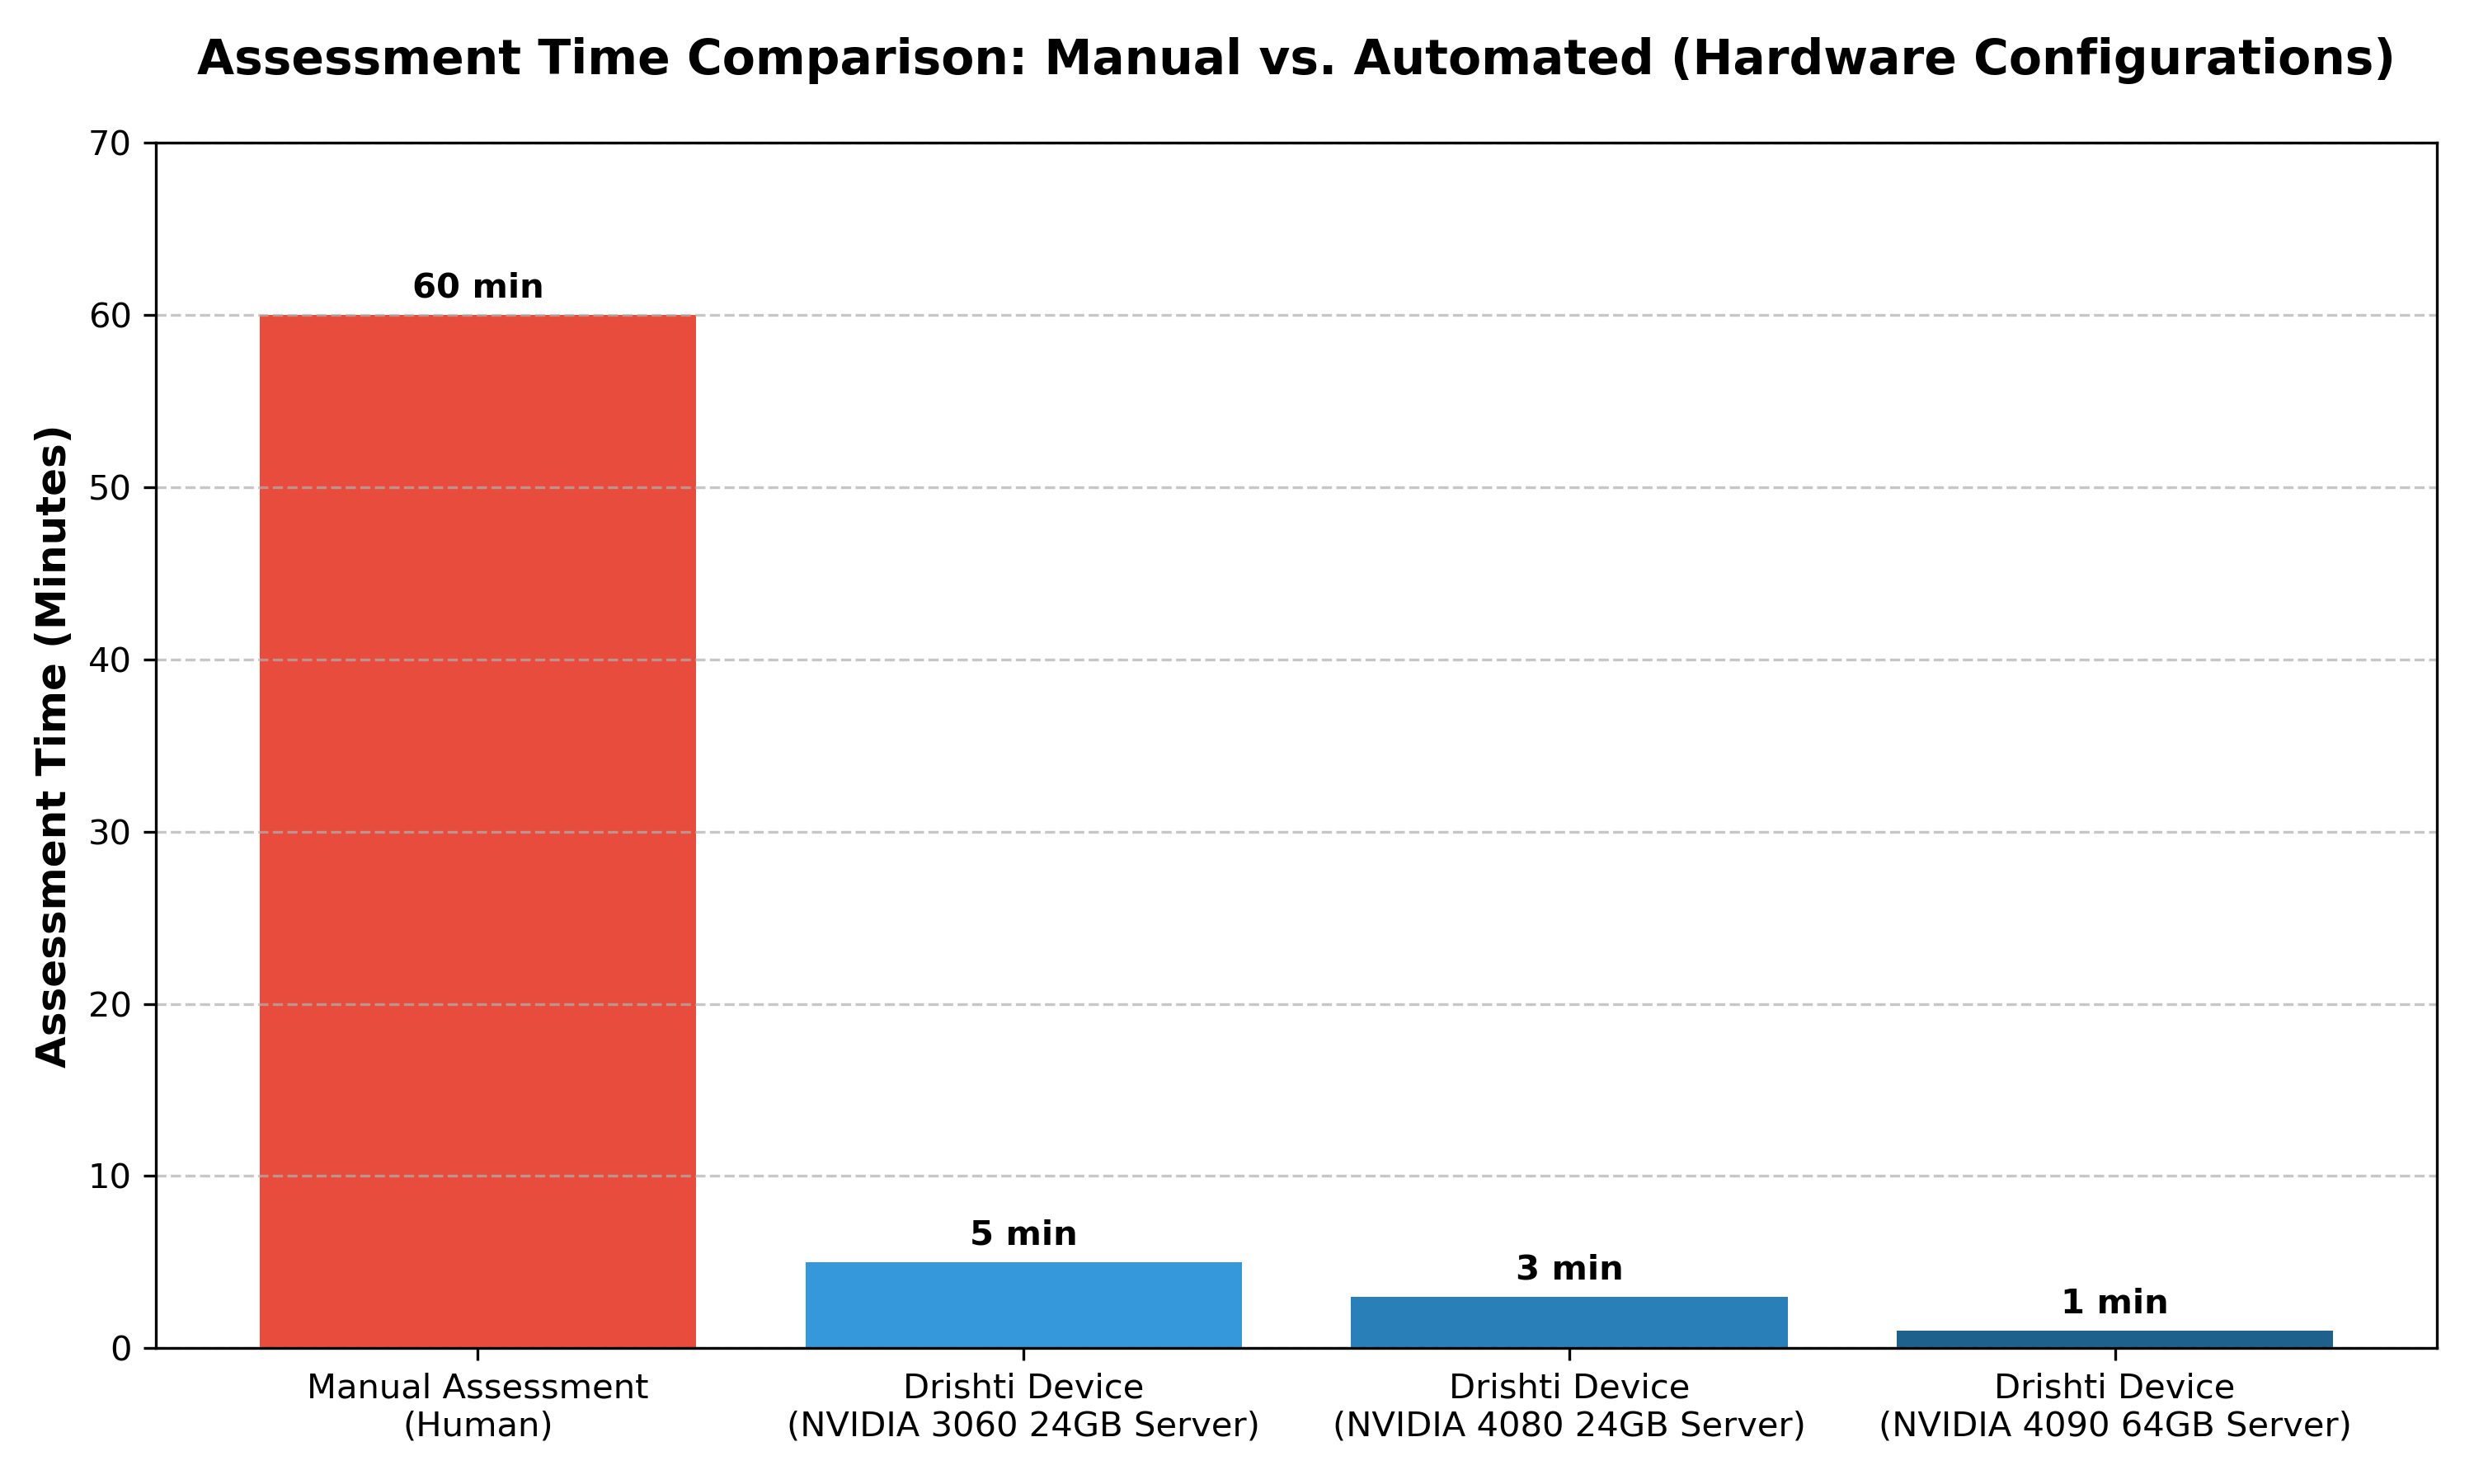
\includegraphics[width=0.95\textwidth]{Images/time_comparison.png}
    \caption{Comparison of assessment times between manual human inspection and the automated Drishti device across various GPU server configurations.}
    \label{fig:time_comparison}
\end{figure}

As illustrated in Figure~\ref{fig:time_comparison}, a baseline deployment using an NVIDIA RTX 3060 (24GB Server) completes the full assessment in approximately 5 minutes. Upgrading to an NVIDIA RTX 4080 (24GB Server) reduces this to 3 minutes, while a high-end NVIDIA RTX 4090 (64GB Server) can process the entire pipeline in just 1 minute. This acceleration represents a paradigm shift for high-volume procurement environments, allowing operations to scale without creating a bottleneck at the quality gate.

The reduction from 60 minutes to under 5 minutes is not merely a convenience improvement; it is a structural change in how procurement logistics can be organised. A shift that previously required a full hour per lot can be completed before the truck queue builds to the point where delays propagate through the supply chain.

%----------------------------------------------------------------------------------------
\section{Evaluation of the Mechanical Dispersion System}
%----------------------------------------------------------------------------------------

% Note to author: Insert quantitative dispersion metrics (coverage percentage
% across frames, mean entity isolation rate, spillage incident rate) when available.

The aspect of the prototype that generated the most immediate interest from evaluators was the solenoid dispersion mechanism. Analysts who had spent years sorting wheat grain manually were quick to identify that the staggered-impulse actuation was doing something that vibration-based systems typically do not: producing genuine grain rotation, not just lateral redistribution. This was noted specifically in the context of \textit{Infested} specimens, where the ventral-side entry marks that are one of the most reliable diagnostic features were described as becoming visible in the image sequence in a way that a static loading would not have supported.

The hole-fitting tray interface was operated by each evaluator without instruction beyond a brief demonstration. The drop-in placement motion, which had been a point of design uncertainty during development, was adopted quickly and generated no negative feedback. Evaluators noted that the absence of rails or latches was an improvement over their expectation---dust management was mentioned explicitly by one quality manager as a practical benefit.

No tray instability or spillage was observed across the demonstration cycles. Full quantitative coverage metrics---percentage of sample entities exposed across the frame sequence, mean isolation rate between actuation cycles---are deferred to the field trial phase.

%----------------------------------------------------------------------------------------
\section{Classification Performance}
%----------------------------------------------------------------------------------------

% Note to author: Insert confusion matrix, per-category precision/recall/F1 scores,
% and comparison against manual assessment baseline when available.

The domain-specific model was evaluated against parallel expert assessment on the same wheat lot samples used in the demonstration. The full statistical analysis is pending; the preliminary observations from Bangalore are recorded here as indicative findings, not final conclusions.

Major category detection---pure wheat, foreign matter including stone and chaff, and premium variety separation---produced outputs that evaluators assessed as consistent with their own manual readings of the same samples. The distinction between \textit{Sharbati} and \textit{Lokwan} specimens, which experienced assessors treat as reliable but junior assessors find difficult, was handled correctly in the cases reviewed during the demonstration.

Performance on orientation-sensitive defect categories was noted as appearing stronger than evaluators had expected from a single-camera system. The food analysts attributed this directly to the multi-frame capture approach, confirming the core hardware-software co-design hypothesis: mechanical exposure of previously occluded surfaces produced observable improvement in the system's ability to detect defects whose diagnostic features are not visible from a static top-down view.

The confusable pairs---\textit{Kernel Burnt} versus dark-variety \textit{Pure Wheat}, early \textit{Infested} versus \textit{Broken}---remain the areas of greatest uncertainty until full quantitative data are available.

\begin{figure}[H]
    \centering
    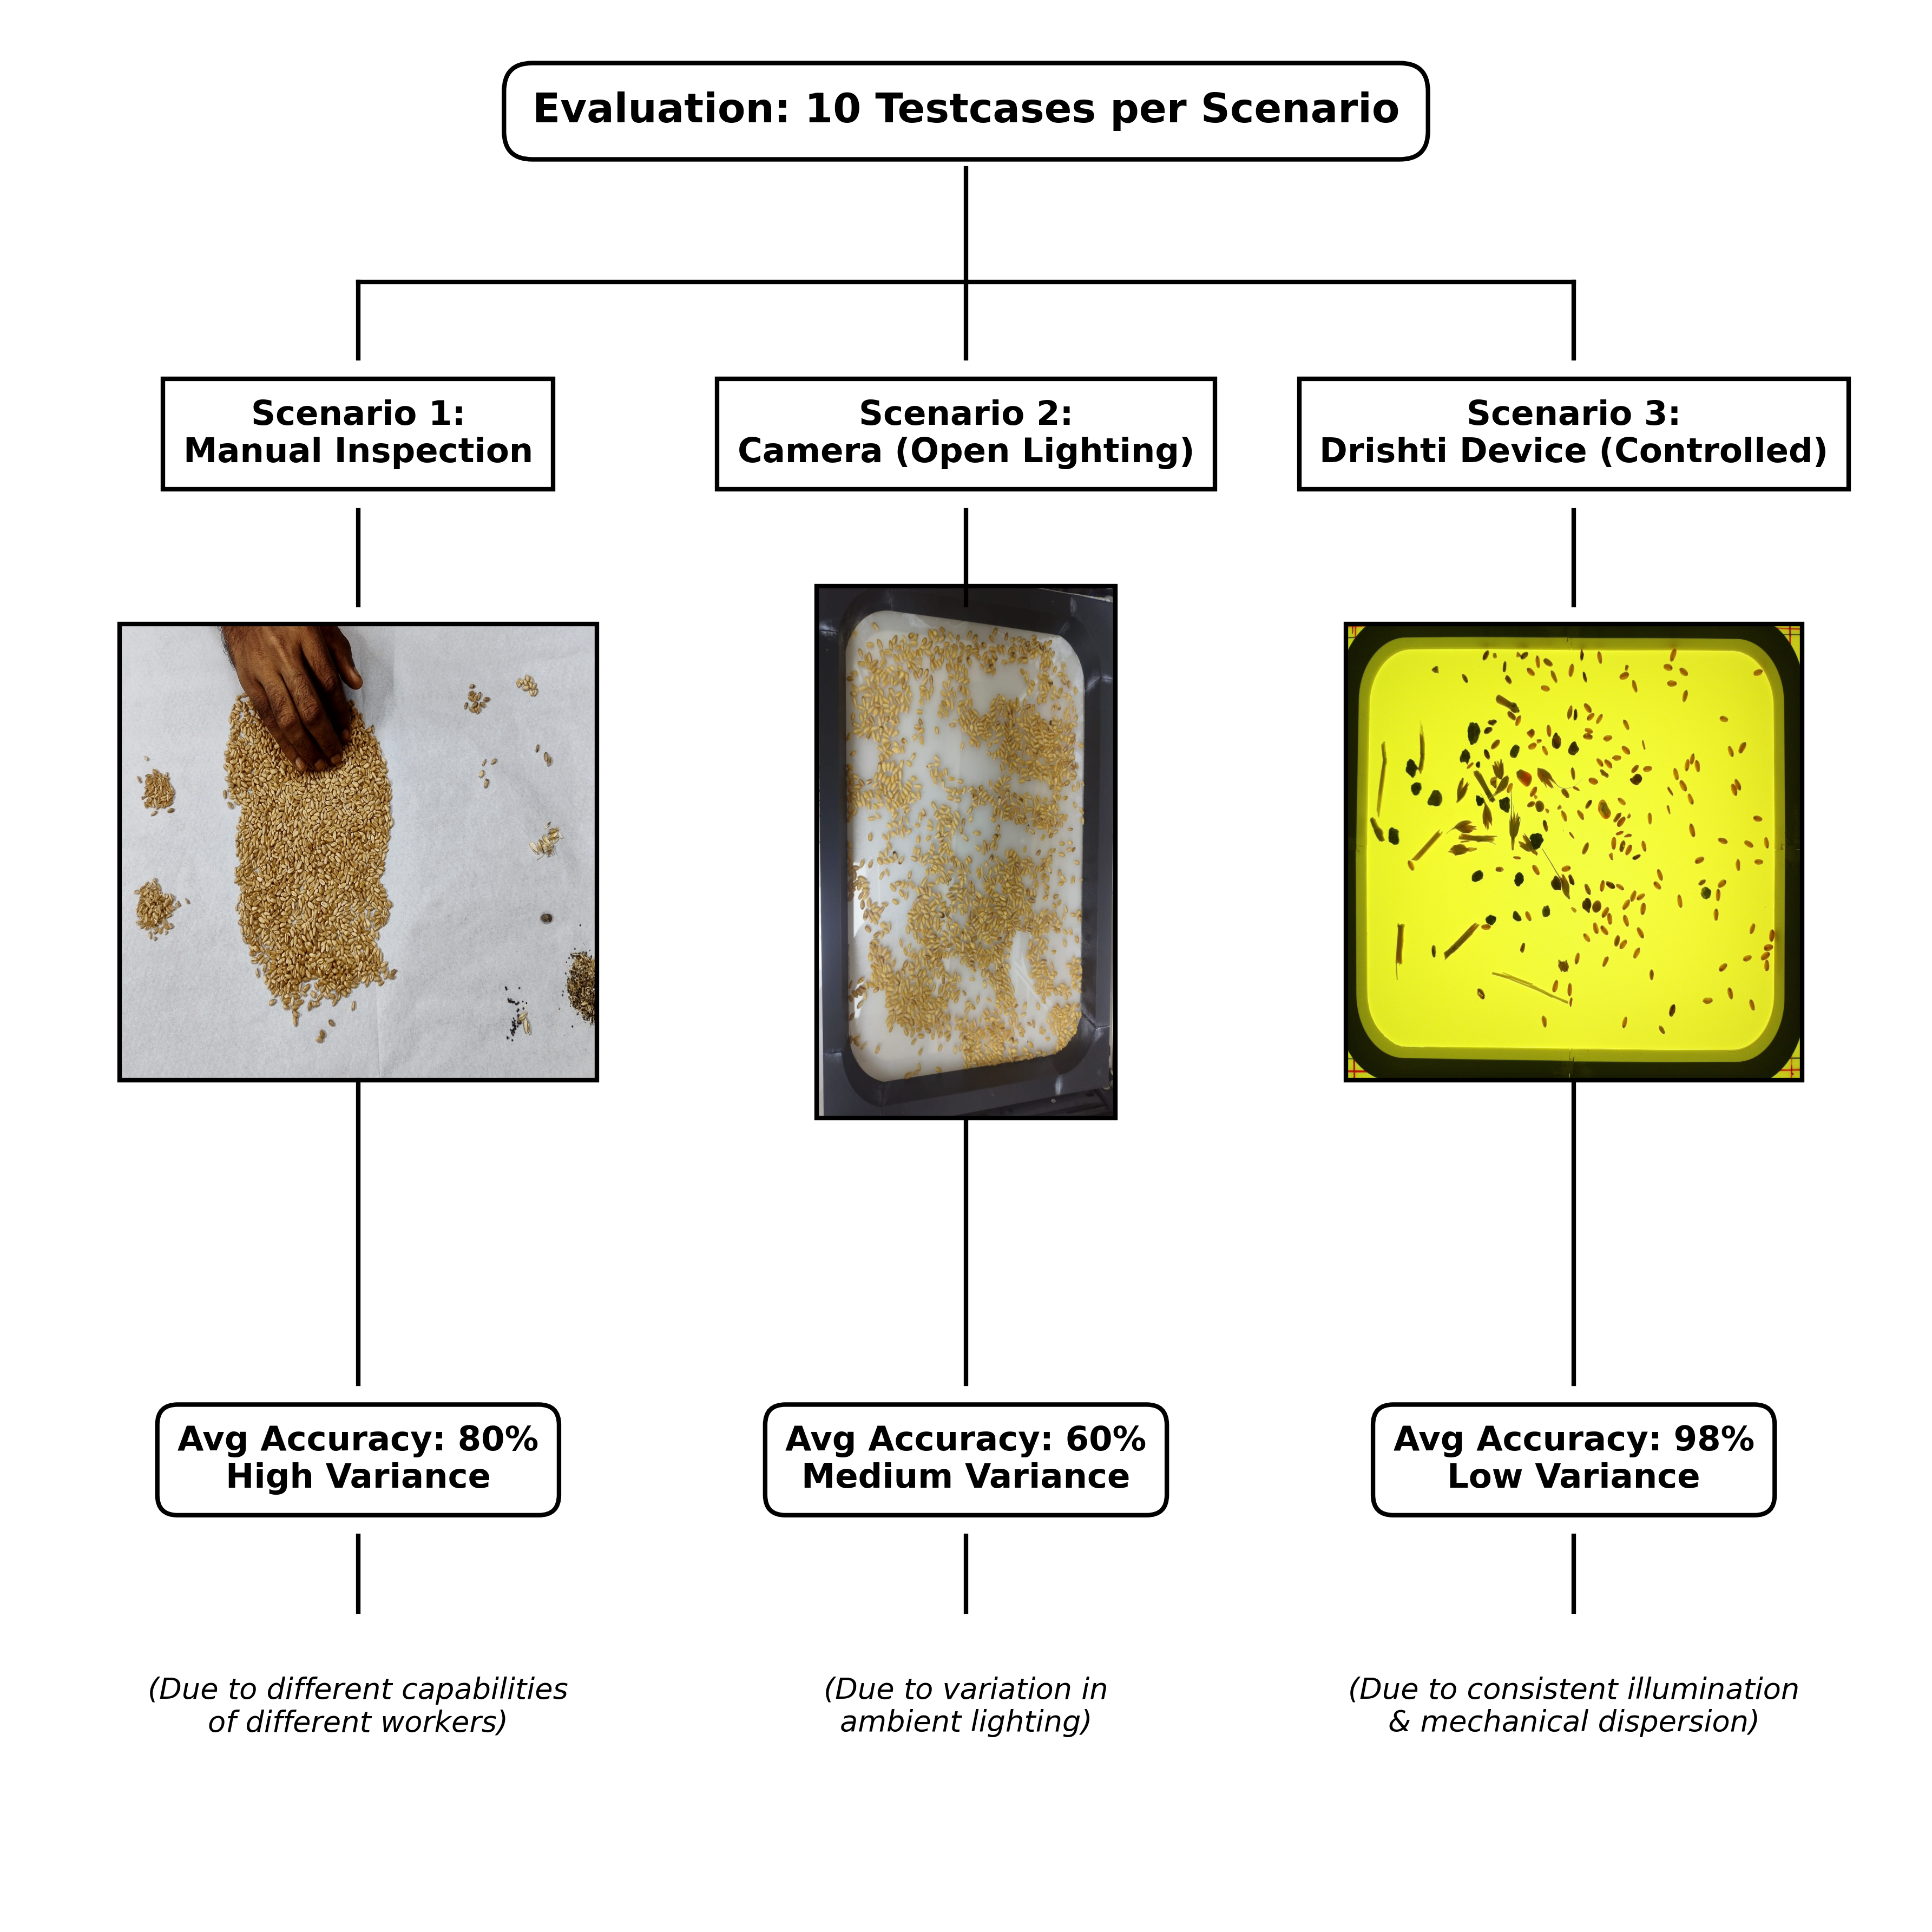
\includegraphics[width=0.95\textwidth]{Images/accuracy_flowchart.png}
    \caption{Comparative accuracy assessment across three inspection scenarios evaluated on ten standard test cases: manual inspection by an experienced technician, camera-based inspection in open uncontrolled lighting, and camera-based inspection within the Drishti device. The Drishti device's controlled illumination and multi-frame capture with solenoid dispersion consistently produced the highest accuracy across defect categories, particularly for orientation-sensitive cases such as Infested and Kernel Burnt grains.}
    \label{fig:accuracy_flowchart}
\end{figure}

%----------------------------------------------------------------------------------------
\section{Expert Feedback: Design and Interface Evaluation}
%----------------------------------------------------------------------------------------

The structured feedback session following the demonstration produced observations across both interaction layers.

On physical handling, the consensus was that tray operation was faster than evaluators had anticipated and that the full cycle sequence was comprehensible without explanation. One evaluator noted that having a device that could be loaded in the same time it takes to walk back to the sorting station was operationally meaningful---a comment that reflects exactly the kind of integration concern that emerged from the fieldwork.

On the digital interface, threshold visualisation was rated more immediately interpretable than the numerical tabular format used in existing warehouse assessment records. The distinction appeared most pronounced among senior managers, who described the threshold-relative indicators as making borderline cases more visible rather than requiring mental comparison of a number against a remembered limit. The Admin Review feature for $\pm 2\%$ threshold samples received explicit approval from senior quality managers, who framed it as consistent with how they already exercise oversight in manual assessment---reviewing borderline calls personally rather than delegating the finalisation of ambiguous results.

%----------------------------------------------------------------------------------------
\section{Summary}
%----------------------------------------------------------------------------------------

The Bangalore evaluation provided early and largely positive evidence for the two central claims of this thesis: that hardware-software co-design can address the physical observability constraints that limit single-image grain assessment, and that field-grounded interface design produces a device that operates meaningfully within the actual workflow rather than alongside it. What the evaluation does not provide, and what should not be claimed from it, is performance certainty across the conditions that matter most for deployment. That requires the multi-site field trials that follow. The Bangalore demonstration is a beginning, not a conclusion.
